\chapter{Soluzione proposta}

La soluzione proposta è suddivisa in due fasi principali:
\begin{itemize}
	\item \textbf{Fase 1}: Suddivisione in caratteri
	\item \textbf{Fase 2}: Classificazione del carattere
\end{itemize}

Per la prima fase vengono utilizzati algoritmi di image processing per suddividere la parola in caratteri. Per la seconda fase viene utilizzato un modello di deep learning per classificare i singoli caratteri.

\begin{figure}[H]
	\centering
	\begin{tikzpicture}[node distance=1.3cm, auto, >=latex, thick]
		% Nodes
		\node[draw, rectangle, rounded corners, fill=blue!10, minimum width=6cm, minimum height=0.7cm] (input) {Immagine in input};
		\node[draw, rectangle, rounded corners, fill=yellow!10, below of=input, minimum width=5cm, minimum height=0.7cm] (preproc) {Preprocessing};
		\node[draw, rectangle, rounded corners, fill=yellow!10, below of=preproc, minimum width=5cm, minimum height=0.7cm] (split) {Suddivisione in caratteri};
		\node[draw, rectangle, rounded corners, fill=orange!10, below of=split, minimum width=5cm, minimum height=0.7cm] (classif) {Classificazione caratteri};
		\node[draw, rectangle, rounded corners, fill=orange!10, below of=classif, minimum width=5cm, minimum height=0.7cm] (heuristics) {Euristiche di correzione};
		\node[draw, rectangle, rounded corners, fill=red!10, below of=heuristics, minimum width=6cm, minimum height=0.7cm] (output) {Testo riconosciuto};

		% Arrows
		\draw[->] (input) -- (preproc);
		\draw[->] (preproc) -- (split);
		\draw[->] (split) -- (classif);
		\draw[->] (classif) -- (heuristics);
		\draw[->] (heuristics) -- (output);

		% Phase labels
		\node[anchor=west] at ($(preproc.east)+(1.2,0)$) {\small \textbf{Fase 1}};
		\node[anchor=west] at ($(split.east)+(1.2,0)$) {\small \textbf{Fase 1}};
		\node[anchor=west] at ($(classif.east)+(1.2,0)$) {\small \textbf{Fase 2}};
		\node[anchor=west] at ($(heuristics.east)+(1.2,0)$) {\small \textbf{Fase 2}};
	\end{tikzpicture}
	\caption{Schema della pipeline di riconoscimento}
	\label{fig:pipeline-schema}
\end{figure}
\section{Fase 1: Suddivisione in caratteri}

Prima di procedere alla suddivisione dell'immagine in singoli caratteri, vengono eseguite alcune operazioni di pre-processing. 

Innanzitutto, l'immagine viene convertita in scala di grigi, così da operare su un unico canale. Successivamente, l'immagine viene normalizzata nell'intervallo 0-255, aumentando così il contrasto tra le aree chiare e scure, migliorando la visibilità dei dettagli. Nel passaggio successivo viene calcolata l'intensità media dei pixel, utile per stimare la luminosità complessiva dell'immagine. Se tale valore supera una soglia prefissata, si assume che l'immagine abbia uno sfondo chiaro; in tal caso, viene applicata un'inversione dei colori, trasformando i pixel chiari in scuri e viceversa. Questa procedura è particolarmente utile perché la rete neurale utilizzata è stata addestrata su immagini con testo bianco su sfondo nero; l'euristica basata sull'intensità media permette quindi di invertire automaticamente i colori, se necessario, per uniformare l'input al formato atteso dalla rete.

Infine, al solo obiettivo di suddividere i caratteri, l'immagine viene convertita in formato binario: attraverso un'operazione di thresholding, i pixel vengono trasformati in nero (0) o bianco (255). Al modello di classificazione verrà poi fornita l'immagine in scala di grigi.
\newline

\begin{figure}[H]
	\centering
	
\includegraphics[width=0.3\textwidth]{images/giraffa-bin.png}
	\caption{Immagine dopo il Preprocessing.}
	\label{fig:giraffabin}
\end{figure}

Il primo approccio utilizzato per la suddivisione in caratteri è stato quello di considerare le proiezioni verticali dell'immagine. Come prima cosa si individuano le colonne in cui è presente almeno un pixel bianco.
L'euristica quindi considera due colonne consecutive come appartenenti allo stesso carattere se presentano entrambe almeno un pixel bianco. Nonostante questo approccio possa sembrare ragionevole, gli esperimenti effettuati mostrano non essere efficaci per immagini a bassa risoluzione. Infatti, in questo caso, i caratteri tendono a sovrapporsi e le colonne consecutive presentano pixel bianchi in comune. Per questo motivo, si è deciso di utilizzare un approccio alternativo.
\newline

L'approccio adottato è quello di considerare le componenti connesse bianche dell'immagine. Questo metodo è più efficace, consentendo di individuare più facilmente caratteri diversi, anche se parzialmente sovrapposti orizzontalmente. L'algoritmo non consente di individuare correttamente i caratteri non contigui, come nel caso di `i` e `j`, che presentano un punto sopra il corpo del carattere. Un'ulteriore euristica risolve il problema in maniera efficace, andando a unire due componenti connesse se parzialmente sovrapposte orizzontalmente. Nello specifico, si prende in considerazione la componente connessa più piccola in larghezza e la si confronta con la parte in sovrapposizione con l'altra componente connessa. Se più del 30\% (valore verificato sperimentalmente) della larghezza è sovrapposto, allora le componenti vengono unite. In questo modo, si riesce a ottenere un'immagine in cui ogni carattere è rappresentato da una singola componente connessa.
\newline

Una volta individuati i bounding box dei caratteri, si procede anche a calcolare un bounding box globale che racchiude tutti i caratteri. L'utilità di questo bounding box viene mostrata nella fase di classificazione.

\begin{figure}[H]
	\centering
	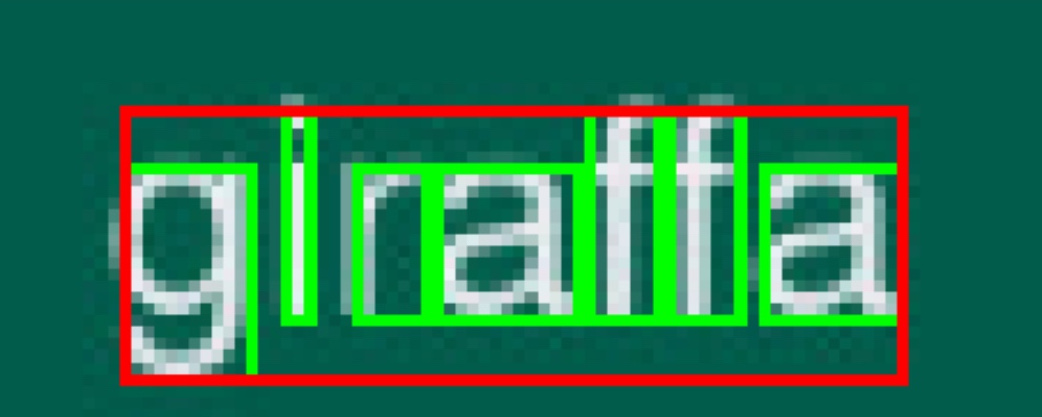
\includegraphics[width=0.3\textwidth]{images/giraffa-bb.jpeg}
	\caption{Individuazione Bounding Box}
	\label{fig:screenshot}
\end{figure}

\section{Fase 2: Classificazione del carattere}

Per la classificazione del carattere viene utilizzato un modello di deep learning. Il modello è stato addestrato su un dataset di immagini di caratteri e simboli in stampatello, con una risoluzione di 28x28 pixel. È quindi necessario ridimensionare i caratteri estratti dalla fase 1 prima di applicare l'inferenza. Il dataset viene approfondito nella sezione dedicata.

Fornendo al modello esclusivamente il carattere ridimensionato, di quest'ultimo verrebbero ignorate la dimensione e la posizione all'interno della parola. Questa semplificazione causerebbe problemi nella classificazione della punteggiatura e di caratteri \emph{confondibili}.

Senza informazioni sulla posizione, il modello non sarebbe in grado di distinguere tra `,` e `'`. Inoltre, non sarebbe in grado di distinguere tra maiuscole e minuscole \emph{confondibili}.
\newline

Per carattere \emph{confondibile} si intende una lettera in cui la rappresentazione in stampatello minuscolo coincide con quella in stampatello maiuscolo, se ridimensionata. Ad esempio, `C` e `c` sono caratteri confondibili, così come `S` e `s`, mentre `A` e `a` non lo sono.
L'insieme dei caratteri confondibili maiuscoli ($\text{CI}$) è definito come segue:
$$\text{CI} = \{C, J, K, O, P, S, U, V, W, X, Z\}$$

Ovviamente la controparte minuscola contiene gli stessi caratteri.

\subsection{Utilizzo del Bounding Box globale}

È possibile utilizzare il bounding box globale per fornire al modello informazioni sulla posizione e la dimensione del carattere all'interno della parola. Partendo dal bounding box del carattere e da quello globale, è possibile estrarre il margine superiore e inferiore del carattere rispetto al bounding box globale. Una volta normalizzati rispetto all'altezza del bounding box globale, il margine superiore e inferiore del carattere possono essere utilizzati come due parametri aggiuntivi per il modello.

Con questo accorgimento, il modello è adesso in grado distinguere tra `,` e `'`. Inoltre, nel caso della parola `Bob`, è in grado di classificare correttamente la `o`. Questo è possibile in quanto il margine superiore della `o` è solo presente nel caso in cui il carattere sia maiuscolo.

\subsection{La necessità di euristiche per il \emph{case}}

Nonostante quest'ultimo approccio possa sembrare efficace, non è sempre in grado di distinguere tra maiuscole e minuscole.
Mostriamo il motivo attraverso un esempio e lo formalizziamo successivamente.
Consideriamo due parole d'esempio:
\begin{itemize}
	\item `Cocco`: la prima lettera non ha margine superiore e inferiore, e deve essere classificata come maiuscola.
	\item `cocco': la prima lettera non ha margine superiore e inferiore, e deve essere classificata come minuscola.
\end{itemize}

Il modello non è quindi in grado di classificare correttamente i caratteri confondibili quando hanno la stessa altezza del bounding box globale.
È necessario utilizzare un'euristica che, confrontando l'altezza dei vari caratteri, sia in grado di \emph{correggere} la forma maiuscola o minuscola del carattere.

Guardando la distribuzione dei caratteri rispetto al loro margine superiore, è possibile notare quando è possibile classificare con certezza i caratteri confondibili.

\begin{figure}[H]
	\centering
	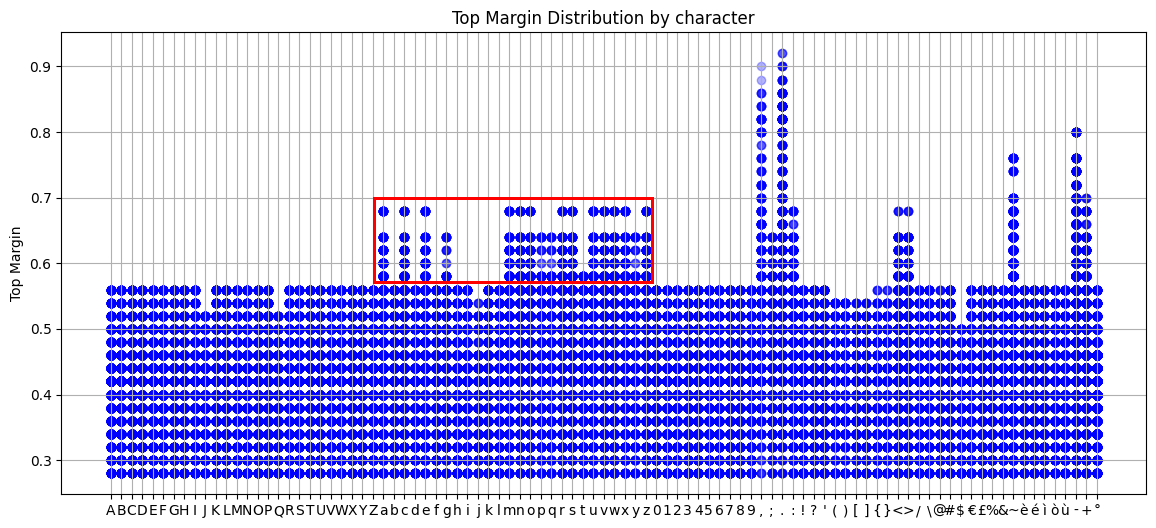
\includegraphics[width=1\textwidth]{images/top_margin_distribution_highlight.png}
	\caption{Distribuzione dei caratteri rispetto al margine superiore. Il rettangolo rosso evidenzia i caratteri confondibili identificabili con affidabilità.}
	\label{fig:top_margin_distribution_highlight.png}
\end{figure}

Rimane comunque il fatto che parole come `COCCO' e `cocco' rimangono indistinguibili anche all'occhio umano, se non affiancate da altre parole che possano disambiguarne il \emph{case}.

\subsection{L'applicazione dell'euristica per il \emph{case}}

Data una determinata immagine, per carattere \emph{affidabile} intendiamo un carattere non confondibile oppure un carattere confondibile di forma minuscola con margine superiore \emph{significativo} (osservando la Figura \ref{fig:top_margin_distribution_highlight.png} si può notare come si aggiri tra il 20\% e il 25\%). Un carattere è quindi affidabile quando la sua interpretazione agli occhi del modello è priva di ambiguità.

L'euristica per la correzione di maiuscole e minuscole può essere applicata solo quando è presente un carattere confondibile la cui altezza coincide con quella del bounding box globale. In questo caso, l'euristica confronta l'altezza del carattere con quella degli altri caratteri affidabili della parola.
L'unico caso in cui l'altezza di un carattere confondibile coincide con quella del bounding box globale è quando non sono presenti caratteri che aumentano l'altezza del bounding box globale. Tra questi sono inclusi tutti i caratteri maiuscoli e qualche carattere minuscolo, come `b`, `d` e `h`.

Ci si potrebbe limitare ad applicare l'euristica nei casi sopra applicati. Purtroppo però, i concetti sopra esposti nella pratica non funzionano. Questo avviene in quanto in ogni font i caratteri minuscoli hanno una proporzione di altezza diversa rispetto ai caratteri maiuscoli. Per questo motivo, l'euristica viene applicata sempre, se possibile, ovvero se è presente almeno un carattere affidabile.

\subsection{Spazi e classi aggiuntive}

La fase 1, utilizzando le componenti connesse, non è in grado di estrarre direttamente gli spazi. Per poterli individuare, è necessario utilizzare delle euristiche aggiuntive. Si considera il margine tra i vari caratteri e sulla base di questo si decide se aggiungere uno spazio o meno. In particolare, viene inserito uno spazio se la distanza tra due caratteri è superiore al 60\% della differenza tra la distanza massima e la minima tra i caratteri. Sperimentalmente, questo valore si è rilevato efficace per frasi di senso compiuto in lingua italiana. Tuttavia, per sequenze di caratteri generate randomicamente, il risultato ottenuto è piuttosto deludente, come approfondito nella sezione dedicata alla valutazione.

Inoltre, le virgolette, essendo composte da due componenti connesse, vengono classificate artificialmente andando a unire una sequenza di due apostrofi consecutivi.